
% !TEX TS-program = XeLaTeX
% !TEX encoding = UTF-8 Unicode

\documentclass[article,pagebackref]{bespoke5}
\usepackage{bespoke5math}
\usepackage{standalone}
%\usepackage[braket, qm]{qcircuit}
\usepackage[flushleft]{threeparttable}
\usepackage{adjustbox}


\newcommand{\thetitle}{Gates, States, and Circuits: \\ \small Notes on the circuit model of quantum computation}
\newcommand{\thesubject}{Gates, States, and Circuits}
\newcommand{\theversion}{2}
\newcommand{\theauthor}{Gavin E.\ Crooks}

\hypersetup{ 
	pdfauthor={Gavin E. Crooks}, 
	pdftitle={\thetitle} ,
	pdfsubject={\thesubject}
}

\setlength{\tabcolsep}{2pt}

\usepackage{tikz}
\usepackage{tikz-3dplot}
\usetikzlibrary{backgrounds,fit,decorations.pathreplacing,shapes}  % TikZ libraries
\tdplotsetmaincoords{80}{35}

\usetikzlibrary{quantikz}


%\newcommand{\sfrac}[2]{\ensuremath{\mathchoice{\tfrac{#1}{#2}}{\tfrac{#1}{#2}}{\frac{#1}{#2}}{\frac{#1}{#2}}}}
%\newcommand{\Gate}[1]{\ensuremath{\sf{#1}}}
\newcommand{\Gate}[1]{\ensuremath{{\sf{#1}}}}
\newcommand{\arxiv}[1]{{arXiv}:\href{http://arxiv.org/abs/#1}{#1}}


\newcommand{\loceq}{\cong}

%\setcounter{secnumdepth}{5}
\setcounter{tocdepth}{5}



\begin{document}
\nocite{???}

\title{\thetitle}
\author{\href{http://threeplusone.com/}{Gavin E.\ Crooks}}
\date{\isotoday}

\preprint{
Tech. Note 014v\theversion ~~~ \href{http://threeplusone.com/gates}{http://threeplusone.com/gates}
}
\maketitle

\tableofcontents


\section{Single qubit gates}


\paragraph{Pauli-I} (identity):\index{I}\index{Pauli-I}\index{identity}

\begin{center}
\input{circuits/I.tex}
%
$\qquad\left(\begin{array}{rr}1 & 0 \\ 0 & 1 \end{array}\right)$
\end{center}



\paragraph{Pauli-X gate} (X-gate, NOT, bit flip)
 
\begin{center}
\input{circuits/X.tex}
%
$\qquad\left(\begin{array}{rr}0 & 1 \\ 1 & 0 \end{array}\right)$
\end{center}

\paragraph{Pauli-Y gate} (Y-gate) :

\begin{center}
\input{circuits/Y.tex}
%
$\qquad\left(\begin{array}{rr} 0 & -i \\ i & 0 \end{array}\right)$
\end{center}

Useful mnemonic: ``Minus eye high''

\paragraph{Pauli-Z gate} (Z-gate, phase flip)

\begin{center}
\input{circuits/Z.tex}
%
$\qquad\left(\begin{array}{rr}1 & 0 \\ 0 & -1 \end{array}\right)$
\end{center}

\paragraph{S} (Phase, P, 'ess') gate

\begin{center}
\input{circuits/S.tex}
%
$\qquad\left(\begin{array}{rr}1 & 0 \\ 0 & i \end{array}\right)$
\end{center}

\paragraph{T} ("tee", $\pi/8$) gate

\begin{center}
\input{circuits/T.tex}
%
$\qquad\Left(\begin{array}{cc}1 & 0 \\ 0 & e^{i \pi/4} \end{array}\Right)$
\end{center}



\paragraph{Hadamard gate}

\begin{center}
\input{circuits/H.tex}
%
$\qquad\begin{bmatrix}1 & 1 \\ 1 & -1 \end{bmatrix}$
\end{center}



$$
\input{circuits/RX.tex}
$$

$$
\input{circuits/RY.tex}
$$

$$
\input{circuits/RZ.tex}
$$

%$$
%\input{circuits/TX.tex}
%$$

%$$
%\input{circuits/TY.tex}
%$$

%$$
%\input{circuits/TZ.tex}
%$$


$$
\input{circuits/ph.tex}
$$

$$
\input{circuits/inv_ph.tex}
$$




%
%\paragraph{pseudo-Hadamard gate}
%
%\begin{center}
%\begin{tikzpicture}[baseline=(op10.base)]
%\draw +(-0.5,0) -- +(+0.5,0);
%\node[U] (op10) {h};
%\end{tikzpicture}
%%
%$\qquad\left(\begin{array}{rr}1 & -1 \\ 1 & 1 \end{array}\right)$
%\end{center}
%
%% J. A. Jones, R. H. Hansen, and M. Mosca, Jl. Magn. Reson., 135, 353 (1998).
%
%\paragraph{inverse pseudo-Hadamard gate}
%
%\begin{center}
%\begin{tikzpicture}[baseline=(op10.base)]
%\draw +(-0.5,0) -- +(+0.5,0);
%\node[U] (op10) {h'};
%\end{tikzpicture}
%%
%$\qquad\left(\begin{array}{rr}1 & 1 \\ -1 & 1 \end{array}\right)$
%\end{center}
%
%\paragraph{V gate} [TODO:CHeck me. Source?] ?????
%
%\begin{center}
%\begin{tikzpicture}[baseline=(op10.base)]
%\draw +(-0.5,0) -- +(+0.5,0);
%\node[U] (op10) {V};
%\end{tikzpicture}
%%
%$
%\qquad
%\tfrac{1}{\sqrt{2}}
%\begin{bmatrix}
% 1+i & 1-i \\
% 1-i & 1+i \\
%\end{bmatrix}
%$
%\end{center}
%
%

\begin{figure}
\begin{center}
 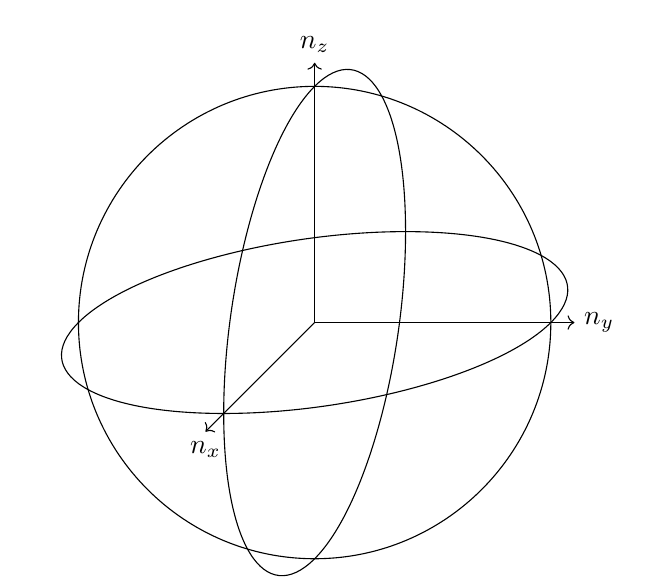
\begin{tikzpicture}[scale=3]
   \begin{scope}[canvas is zy plane at x=0]
     \draw (0,0) circle (1cm);
     %\draw[ultra thin] (-1,0) -- (1,0) (0,-1) -- (0,1);
     \draw[->] (0,0) -- (1.2,0) node[below ] {$n_x$};
   \end{scope}

   \begin{scope}[canvas is zx plane at y=0]
     \draw (0,0) circle (1cm);
     %\draw (-1,0) -- (1,0) (0,-1) -- (0,1);
     \draw[->] (0,0) -- (0,1.1) node[right] {$n_y$};
   \end{scope}

   \begin{scope}[canvas is xy plane at z=0]
     \draw (0,0) circle (1cm);
	%\draw (-1,0) -- (1,0) (0,-1) -- (0,1);
	\draw[->] (0,0) -- (0,1.1) node[above] {$n_z$};
   \end{scope}

	 
 \end{tikzpicture}
 \end{center}
\caption{Sphere of 1-qubit gates. Each point within this sphere represents a unique (up to phase) 1-qubit gate. 
Antipodal points on the surface represent the same gate.}
\end{figure}


\begin{figure}
\begin{center}
 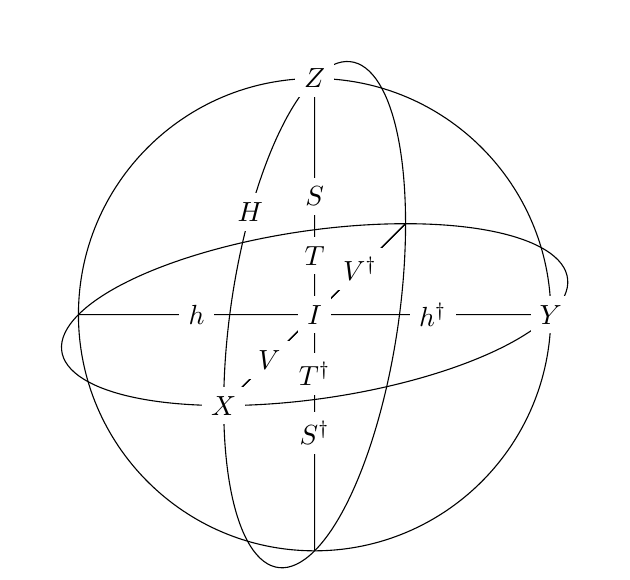
\begin{tikzpicture}[scale=3]
   \begin{scope}[canvas is zy plane at x=0]
     \draw (0,0) circle (1cm);
     \draw (-1,0) -- (1,0) (0,-1) -- (0,1);
   \end{scope}

   \begin{scope}[canvas is zx plane at y=0]
     \draw (0,0) circle (1cm);
     \draw (-1,0) -- (1,0) (0,-1) -- (0,1);
   \end{scope}

   \begin{scope}[canvas is xy plane at z=0]
     \draw (0,0) circle (1cm);
     \draw (-1,0) -- (1,0) (0,-1) -- (0,1);
   \end{scope}

	\node[fill=white] at (0,0,0) {$I$};

	\node[fill=white] at (0,1,0) {$Z$};
	\node[fill=white] at (0,0.5,0) {$S$};
	\node[fill=white] at (0,0.25,0) {$T$};			
	\node[fill=white] at (0,-0.5,0) {${S^\dagger}$};
	\node[fill=white] at (0,-0.25,0) {$T^\dagger$};	
	% \node[fill=white] at (0,-1,0) {Z};
		
	\node[fill=white] at (0,0,1) {$X$};
	\node[fill=white] at (0,0,0.5) {$V$};
	\node[fill=white] at (0,0,-0.5) {$V^\dagger$};	
	% \node[fill=white] at (0,0,-1) {X};
	
	\node[fill=white] at (0,{sqrt(1/2)},{sqrt(1/2)}) {$H$};
%	\node[fill=white] at (0,0,1) {H};
	
	\node[fill=white] at (1,0,0) {$Y$};
	\node[fill=white] at (0.5,0,0) {${h^\dagger}$};	
	\node[fill=white] at (-0.5,0,0) {${h}$};	
	% \node[fill=white] at (-1,0,0) {$Y$};
 \end{tikzpicture}
 \end{center}
\caption{Coordinates of common 1-qubit gates}
\end{figure}




\begin{figure*}

% !TEX TS-program = XeLaTeX
% !TEX encoding = UTF-8 Unicode

\documentclass[border=10pt]{standalone}

\usepackage[dvipsnames]{xcolor}	    % Load before tikz
\usepackage[hidelinks]{hyperref}
\usepackage{tikz, tkz-euclide} 
\usepackage{qcircuit}

\usepackage{fontspec}
\usepackage[OT1]{fontenc}

\usepackage{eulervm} 				% Load before amssymb
\usepackage{amsmath}
\usepackage{amssymb}


\IfFontExistsTF{Trump Mediaeval LT Std}{%
	\setromanfont[Mapping=tex-text, Scale=0.95, AutoFakeSlant]{Trump Mediaeval LT Std}
}

\overfullrule=1mm

\newcommand{\thetitle}{On the Weyl chamber of Canonical 2-qubit quantum gates}
\hypersetup{ 
	pdfauthor={Gavin E. Crooks}, 
	pdftitle={\thetitle} ,
}

\newcommand{\Gate}[1]{{\sf{#1}}}

\begin{document}


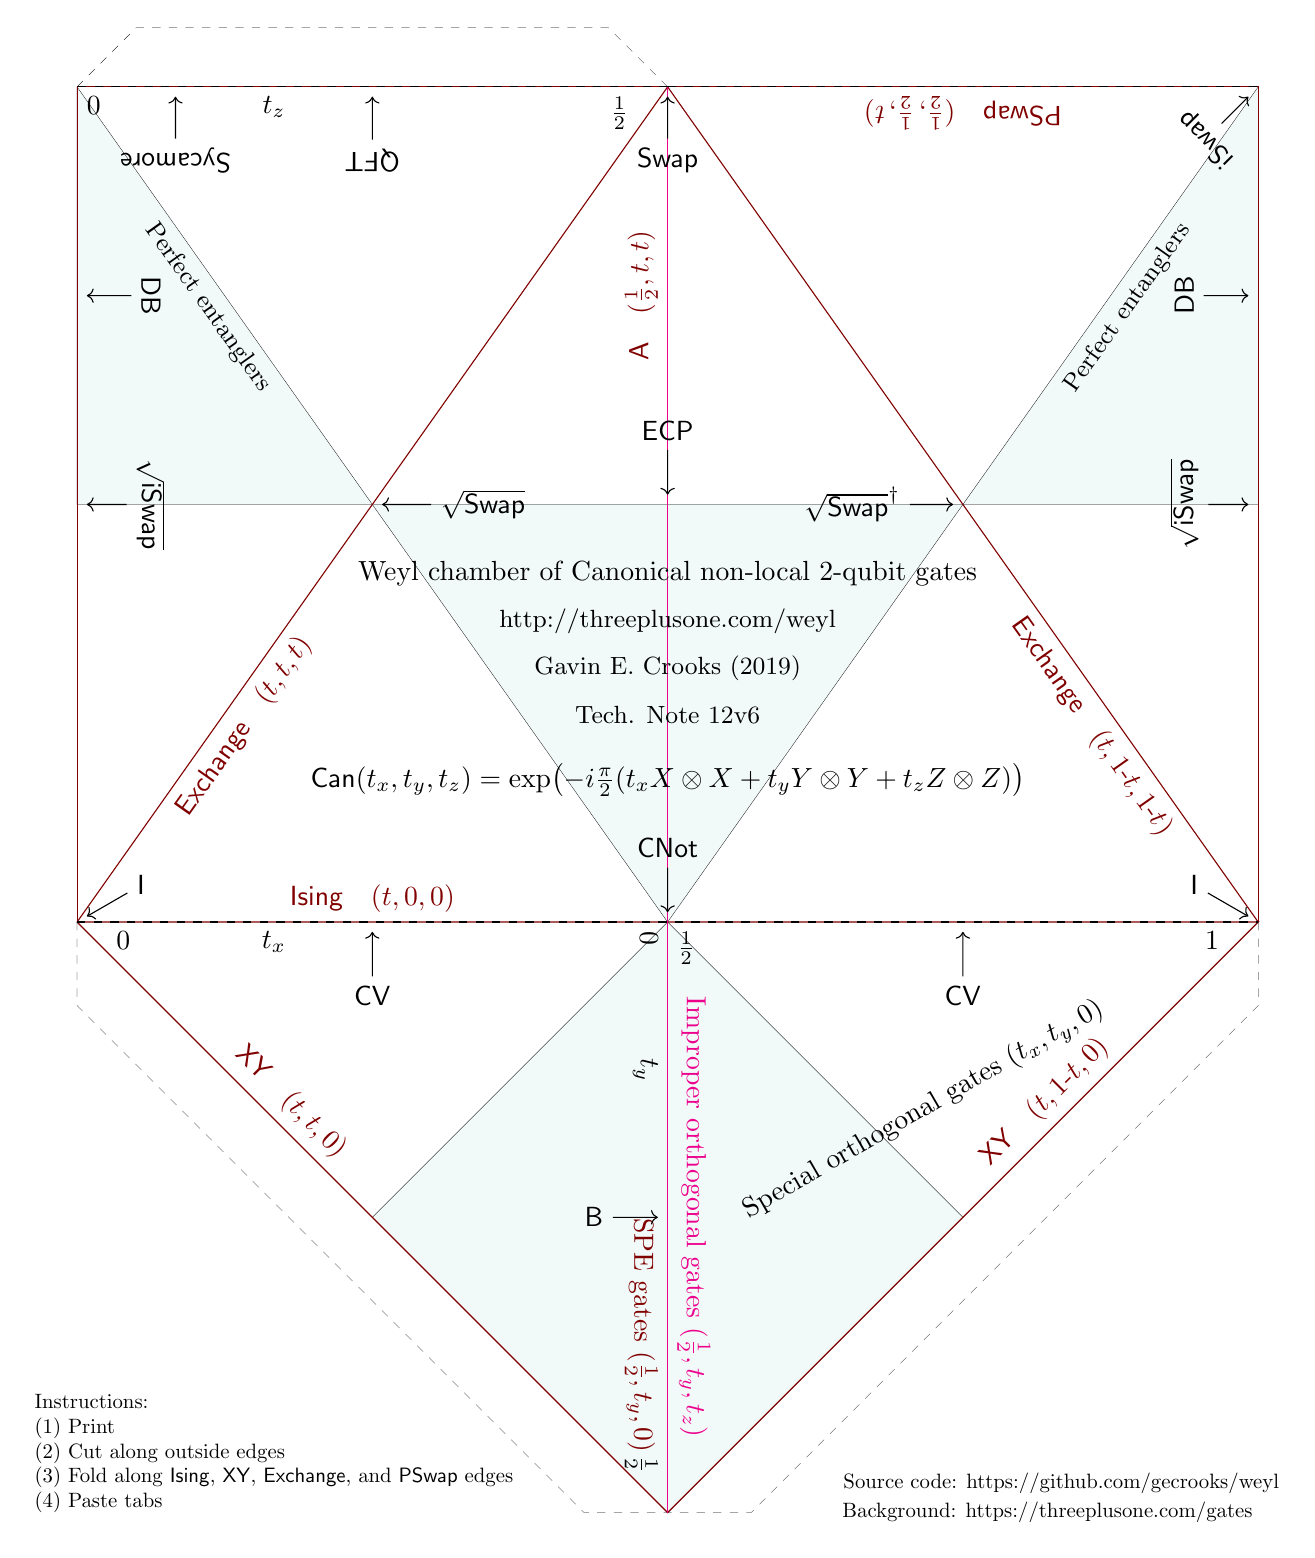
\begin{tikzpicture}[scale=7.5]

\def\sep{0.125}  % Separation between gates and gate labels
\def\ang{54.74} % = arctan(sqrt(2)) in degrees, angle of EXCHANGE line 


% Perfect entanglers
\draw [ultra thin, fill=teal!5] (1, 0) -- ({1/2}, {sqrt(2)/2}) -- ({3/2}, {sqrt(2)/2}) -- (1, 0);
\draw [ultra thin, fill=teal!5] (0, {sqrt(2)}) -- ({1/2}, {sqrt(2)/2}) -- (0, {sqrt(2)/2}) -- (0, {sqrt(2)});
\draw [ultra thin, fill=teal!5] (2, {sqrt(2)}) -- ({3/2}, {sqrt(2)/2}) -- (2, {sqrt(2)/2}) -- (2, {sqrt(2)});
\draw [ultra thin, fill=teal!5] (1, 0) -- ({1/2}, {-1/2}) -- (1, -1) --   ({3/2}, {-1/2}) -- (1, 0);

\node [below, rotate=-\ang] at ({1/4}, {sqrt(2)*3/4}) {\small{Perfect entanglers}};
\node [below, rotate= \ang] at ({7/4}, {sqrt(2)*3/4}) {\small{Perfect entanglers}};



% Draw boundary
\draw [Maroon] (0,0) -- (2, 0) -- (1,-1) -- (0,0); 					% Bottom triangle
\draw [Maroon] (0,0) -- (1, {sqrt(2)}) -- (2, 0); 					% Top triangle
\draw [Maroon] (0,0) -- (0, {sqrt(2)}) -- (2, {sqrt(2)}) -- (2,0);	% Upper rectangle


% Draw tabs
\def\tabsize{0.1};					
\draw [ultra thin, dashed] (0, {sqrt(2)}) 
						-- (0 + \tabsize, {sqrt(2) + \tabsize}) 
						-- (1 - \tabsize, {sqrt(2) + \tabsize})
						-- (1, {sqrt(2)});
\draw [ultra thin, dashed] (0, 0) 
						-- (0, {0 - sqrt(2) * \tabsize}) 
						-- ({1 - sqrt(2) * \tabsize}, -1)
						-- (1, -1);
\draw [ultra thin, dashed] (2, 0) 
						-- (2, {0 - sqrt(2) * \tabsize}) 
						-- ({1 + sqrt(2) * \tabsize}, -1)
						-- (1, -1);



% Axes
\draw [dashed,  ] (0, 0) -- (2, 0);
\draw [dashed,  ] (1, {sqrt(2)}) -- (0, {sqrt(2)});
\draw [dashed,  ] (1, {sqrt(2)}) -- (2, {sqrt(2)});
\draw [dashed,  ] (1, 0) -- (1, -1);

\node [below right] at (0+0.05, 0) {$0$};
\node [below] at ({1/3}, 0) {$t_x$};
\node [below right] at (1, 0) {$\tfrac{1}{2}$};
\node [below left] at (2-0.05, 0) {$1$};

\node [below right, rotate=-90] at (1, 0) {$0$};
\node [below, rotate=-90] at (1, -{1/4}) {$t_y$};
\node [below left, rotate=-90] at (1, -1+0.05) {$\tfrac{1}{2}$};

\node [below right] at (0, {sqrt(2)}) {$0$};
\node [below] at ({1/3}, {sqrt(2)}) {$t_z$};
\node [below left] at (1-0.05, {sqrt(2)}) {$\tfrac{1}{2}$};


%% Gate families

% Orthogonal gates
\draw [ultra thin, magenta] (1,0) -- (1, {sqrt(2)});
\draw [ultra thin, magenta] (1,0) -- (1, -1);
\node [above, rotate=-90, magenta] at (1, -{1/2}) {Improper orthogonal gates $(\tfrac{1}{2}, t_y, t_z)$};
\node [above, rotate=30] at ({0.1+ 1+sqrt(2)/4}, -{sqrt(2)/4}) {Special orthogonal gates $(t_x, t_y, 0)$};
\node [below, rotate=-90, Maroon] at (1, -{0.7}) {SPE gates $(\tfrac{1}{2}, t_y, 0)$};


% CPHASE
\node [above, Maroon] at ({1/2}, 0) {$\Gate{Ising}\quad(t,0,0)$};

% XY
\node [above, Maroon, rotate=-45] at ({1/3}, {-1/3}) {$\Gate{XY}\quad(t,t,0)$};
\node [above, Maroon, rotate=45] at ({2-1/3}, {-1/3}) {$\Gate{XY}\quad(t,1$-$t,0)$};

% EXCHANGE
\node [below, Maroon, rotate=\ang] at ({1/4}, {sqrt(2)/4}) {$\Gate{Exchange}\quad(t,t,t)$};
\node [below, Maroon, rotate=-\ang] at ({2-1/4}, {sqrt(2)/4}) {$\Gate{Exchange}\quad(t,1$-$t,1$-$t)$};

% PSWAP
\node [above, Maroon, rotate=180] at ({3/2}, {sqrt(2)}) {$\Gate{PSwap}\quad(\tfrac{1}{2},\tfrac{1}{2},t)$};

% A
\node [above, Maroon, rotate=90] at ({1}, {3*sqrt(2)/4}) {$\Gate{A}\quad(\tfrac{1}{2},t,t)$};



%% Gate Nodes
\node (I) 		at (0, 0) {};
\node (I_L) 	at ([shift={(30:\sep)}]I) {\Gate{I}};
\draw [->] (I_L) -- (I);

\node (I2) 		at (2, 0) {};
\node (I2_L) 	at ([shift={(150:\sep)}]I2) {\Gate{I}};
\draw [->] (I2_L) -- (I2);

\node (CNOT) 	at (1, 0) {};
\node (CNOT_L) 	at ([shift={(90:\sep)}]CNOT) {\Gate{CNot}};
\draw[->] (CNOT_L) -- (CNOT);

\node (SWAP) 	at (1, {sqrt(2)}) {};
\node (SWAP_L) at ([shift={(270:\sep)}]SWAP) {$\Gate{Swap}$};
\draw[->] (SWAP_L) -- (SWAP);

\node (SWAPR) 	at ({1/2}, {sqrt(2)/2}) {};			% Root of SWAP
\node (SWAPR_L) at ([shift={(0:{\sep*3/2})}]SWAPR) {$\sqrt{\Gate{Swap}}$};
\draw[->] (SWAPR_L) -- (SWAPR);

\node (SWAPRI) 	at ({3/2}, {sqrt(2)/2})	{};			% SWAP, Sqrt, inverse
\node (SWAPRI_L) at ([shift={(180:{\sep*3/2})}]SWAPRI) {$\sqrt{\Gate{Swap}}^\dagger$};
\draw[->] (SWAPRI_L) -- (SWAPRI);

\node (ECP)		at (1, {sqrt(2)/2}) {};
\node (ECP_L) at ([shift={(90:\sep)}]ECP) {${\Gate{ECP}}$};
\draw[->] (ECP_L) -- (ECP);

\node (B)		at (1, {-1/2}) {};
\node (B_L) at ([shift={(0:-\sep)}]B) {${\Gate{B}}$};
\draw[->] (B_L) -- (B);

\node (ISWAP) at (0, {sqrt(2)}) {};
\node (ISWAP2)	at (2, {sqrt(2)}) {};
\node [rotate=135] (ISWAP2_L) at ([shift={(225:\sep)}]ISWAP2) {${\Gate{iSwap}}$};
\draw[->] (ISWAP2_L) -- (ISWAP2);

\node (ISWAPR)	at (0, {sqrt(2)/2}) {};
\node [rotate=270] (ISWAPR_L) at ([shift={(0:\sep)}]ISWAPR) {$\sqrt{\Gate{iSwap}}$};
\draw[->] (ISWAPR_L) -- (ISWAPR);

\node (ISWAPR2)	at (2, {sqrt(2)/2}) {};
\node [rotate=90] (ISWAPR2_L) at ([shift={(180:\sep)}]ISWAPR2) {$\sqrt{\Gate{iSwap}}$};
\draw[->] (ISWAPR2_L) -- (ISWAPR2);

\node (DB) at (0, {sqrt(2)*3/4}) {};
\node [rotate=270] (DB_L) at ([shift={(0:\sep)}]DB) {${\Gate{DB}}$};
\draw[->] (DB_L) -- (DB);

\node (DB2) at (2, {sqrt(2)*3/4}) {};
\node [rotate=90] (DB2_L) at ([shift={(180:\sep)}]DB2) {${\Gate{DB}}$};
\draw[->] (DB2_L) -- (DB2);

\node (QFT)		at ({1/2}, {sqrt(2)}) {};
\node [rotate=180] (QFT_L) at ([shift={(270:\sep)}]QFT) {${\Gate{QFT}}$};
\draw[->] (QFT_L) -- (QFT);

\node (QFT2) at ({3/2}, {sqrt(2)}) {};

\node (SYC)		at ({1/6}, {sqrt(2)}) {};
\node [rotate=180] (SYC_L) at ([shift={(270:\sep)}]SYC) {${\Gate{Sycamore}}$};
\draw[->] (SYC_L) -- (SYC);


\node (CNOTR) at ({1/2}, 0) {};
\node (CNOTR_L) at ([shift={(270:\sep)}]CNOTR) {$\Gate{CV}$};
\draw[->] (CNOTR_L) -- (CNOTR);

\node (CNOTR2)	at ({3/2}, 0) {};
\node (CNOTR2_L) at ([shift={(270:\sep)}]CNOTR2) {$\Gate{CV}$};
\draw[->] (CNOTR2_L) -- (CNOTR2);


\node at (1, 0.59){Weyl chamber of Canonical non-local 2-qubit gates};
\node at (1, 0.51){\small{\url{http://threeplusone.com/weyl}}};
\node at (1, 0.43){\small{Gavin E. Crooks (2019)}};
\node at (1, 0.35){\small{Tech. Note 12v6}};


\node at (1,0.24){$\Gate{Can}(t_x, t_y, t_z)  = \exp\bigl(-i\frac{\pi}{2}
	(t_x X\otimes X + t_y Y\otimes Y + t_z Z \otimes Z) \bigr)$};


\node[align=left, scale=0.75] at ({1/3}, -0.9) {
	Instructions:\\
	(1) Print\\
	(2) Cut along outside edges\\
	(3) Fold along \Gate{Ising}, \Gate{XY}, \Gate{Exchange}, and \Gate{PSwap} edges\\
	(4) Paste tabs
};

\node[align=left,, scale=0.75] at ({5/3}, -0.95) {Source code: \url{https://github.com/gecrooks/weyl}};
\node[align=left,, scale=0.75] at ({5/3}, -1.00) {Background: \url{https://threeplusone.com/gates}~~~~};


\end{tikzpicture}


\end{document}

\caption{The Weyl chamber of canonical non-local 2 qubit gates. (Print, cut, fold, and paste)}
\label{weyl_fig}
\end{figure*}

\begin{figure*}[tp]
\begin{center}
\begin{tikzpicture}[tdplot_main_coords, scale=7.5]
\draw (0,0,0) -- (2,0,0) -- (1,1,0)  -- cycle
      (0,0,0) -- (1,1,1) -- (1,1,0)  -- cycle
      (2,0,0) -- (1,1,1) -- (1,1,0)  -- cycle
      (2,0,0) -- (1,1,1) -- (1,1,0)  -- cycle;
\draw (1,0,0) -- (1,1,0) -- (1,1,1) -- cycle;
%\draw [ultra thick, Maroon] (0, 0, 0) -- (1,1,1) -- (2, 0, 0);

\node (SWAP) at (1, 1, 1) {};
\node (SWAP_L) at (1+0.25, 1, 1) {${\Gate{SWAP}}$};
\draw[thin, ->] (SWAP_L) -- (SWAP);

\node (SRSWAP) at (0.5, 0.5, 0.5) {};
\node (SRSWAP_L) at (0.5-0.25, 0.5, 0.5) {${\Gate{\sqrt{SWAP}}}$};
\draw[ultra thin, ->] (SRSWAP_L) -- (SRSWAP);

\node (SRSWAPI) at (1.5, 0.5, 0.5) {};
\node (SRSWAPI_L) at (1.5+0.25, 0.5, 0.5) {${\Gate{\sqrt{SWAP}^\dagger}}$};
\draw[ultra thin, ->] (SRSWAPI_L) -- (SRSWAPI);

\node (I2) at (2, 0, 0) {};
\node (I2_L) at (2, 0, -0.25) {${{I}}$};
\draw[ultra thin, ->] (I2_L) -- (I2);

\node (I) at (0, 0, 0) {};
\node (I_L) at (0, 0, -0.25) {${{I}}$};
\draw[ultra thin, ->] (I_L) -- (I);

\node (CNOT) at (1, 0, 0) {};
\node (CNOT_L) at (1, 0, -0.25) {${\Gate{CNOT}}$};
\draw[ultra thin, ->] (CNOT_L) -- (CNOT);

\node (SRCNOT) at (0.5, 0, 0) {};
\node (SRCNOT_L) at (0.5, 0, -0.25) {${\Gate{CV}}$};
\draw[ultra thin, ->] (SRCNOT_L) -- (SRCNOT);

\node (SRCNOT2) at (1.5, 0, 0) {};
\node (SRCNOT2_L) at (1.5, 0, -0.25) {${\Gate{CV}}$};
\draw[ultra thin, ->] (SRCNOT2_L) -- (SRCNOT2);

\node (iSWAP) at (1, 1, 0) {};
\node (iSWAP_L) at (1, 1, -0.25) {${\Gate{iSWAP}}$};
\draw[ultra thin, ->] (iSWAP_L) -- (iSWAP);

\node (B) at (1, 0.5, 0) {};
\node (B_L) at (1, 0.5, -0.25) {${\Gate{B}}$};
\draw[ultra thin, ->] (B_L) -- (B);

\node (ECP) at (1, 0.5, 0.5) {};
\node (ECP_L) at (1-0.25, 0.5, 0.5) {${\Gate{ECP}}$};
\draw[ultra thin, ->] (ECP_L) -- (ECP);

\node (QFT) at (1, 1, 0.5) {};
\node (QFT_L) at (1+0.25, 1, 0.5) {${\Gate{QFT}}$};
\draw[ultra thin, ->] (QFT_L) -- (QFT);

\node (SRiSWAP) at (0.5, 0.5, 0) {};
\node (SRiSWAP_L) at (0.5, 0.5, -0.25) {${\Gate{\sqrt{iSWAP}}}$};
\draw[ultra thin, ->] (SRiSWAP_L) -- (SRiSWAP);

\node (SRiSWAP2) at (1.5, 0.5, 0) {};
\node (SRiSWAP2_L) at (1.5, 0.5, -0.25) {${\Gate{\sqrt{iSWAP}}}$};
\draw[ultra thin, ->] (SRiSWAP2_L) -- (SRiSWAP2);

\draw[thick,->] (0,0,0) -- (0.25,0,0) node[anchor=north east]{${t_x}$};
\draw[thick,->] (0,0,0) -- (0,0.25,0) node[anchor= west]{${t_y}$};
\draw[thick,->] (0,0,0) -- (0,0,0.25) node[anchor=south]{${t_z}$};

\end{tikzpicture}
\end{center}

\caption{Location of the 11 principal 2-qubit gates in the Weyl chamber. All of these gates have coordinates of the form $\Gate{CAN}(\sfrac{1}{4}k_x, \sfrac{1}{4}k_y, \sfrac{1}{4}k_z)$, for integer $k_x$, $k_y$, and $k_z$.
Note there is a symmetry on the bottom face such that $CAN(t_x, t_y, 0) \loceq CAN(\half-t_x, t_y, 0)$.
}
\end{figure*}



\section{The canonical gate}
The canonical gate is a 3-parameter quantum logic gate that acts on two qubits.
\[
\Gate{CAN}&(t_x, t_y, t_z) 
\notag \\ = 
&\exp\Bigl(-i\frac{\pi}{2}  (t_x X\otimes X + t_y Y\otimes Y + t_z Z \otimes Z) \Bigr)
\]
Here, $X=(\begin{smallmatrix}0 & 1 \\ 1 & 0\end{smallmatrix})$,
$Y=(\begin{smallmatrix}0 & \text{-}i \\ i & 0\end{smallmatrix})$, 
and $Z=(\begin{smallmatrix}1 & 0 \\ 0 & \text{-}1\end{smallmatrix})$ are the 1-qubit Pauli matrices.
Note that other choices for the prefactor in the exponential are also common in the literature.

The canonical gate is, in a sense, the elementary 2-qubit gate, since any other 2-qubit gate can be decomposed into a canonical gate, and
local 1-qubit interactions~\cite{Zhang2003a,Zhang2004a,Blaauboer2008a,Watts2013a}.
%\[
%\label{canonical}
%\text{\small
%\Qcircuit @C=0.5em @R=1em {
%  & \multigate{1}{U_0} & \qw & & \dstick{\simeq} & &
%  & \gate{U_1}
%  & \multigate{1}{\Gate{CAN}(t_x, t_y, t_z)}
%  & \gate{U_3}
%  & \qw
%  \\
%    & \ghost{U_0} & \qw & &  & &
% & \gate{U_2} 
% & \ghost{\Gate{CAN}(t_7, t_8, t_9)}
% & \gate{U_4} 
%& \qw
%}}
%\]
%
$$
\adjustbox{scale=0.9}{\begin{quantikz}[thin lines, column sep=0.75em, row sep={2.5em,between origins}]
& \gate[2]{U_0} & \qw \\
&  & \qw
\end{quantikz}}
\simeq
\adjustbox{scale=0.9}{\begin{quantikz}[thin lines, column sep=0.75em, row sep={2.5em,between origins}]
& \gate{U_1} & \gate[2]{CAN(t_x, t_y, t_z)} & \gate{U_3} & \qw \\
& \gate{U_2} &                             & \gate{U_4} & \qw
\end{quantikz}}
$$


Here we use '$\simeq$' to indicate that two gates have the same unitary operator up to a global (and generally irrelevant) phase factor.

The canonical gate is periodic in each parameters with period 4, or period 2 if we neglect a $-1$ global phase factor. Thus we can constrain each parameter to the range $[-1,1)$. Since $X\otimes X$,  $Y\otimes Y$, and $Z \otimes Z$ all commute, the parameter space has the topology of a 3-torus.

However, the canonical coordinates of any given 2-qubit gate are not unique since we have considerable freedom in the prepended and postpended local gates. To remove these symmetries we can constraint the canonical parameters to a ``Weyl chamber''~\cite{???,???}.
\begin{equation}
(\tfrac{1}{2} \ge  t_x \ge t_y \ge t_z \ge 0) \cup (\tfrac{1}{2} \ge (1-t_x) \ge t_y \ge t_z > 0 )
\label{WeylChamber}
\end{equation}
This Weyl chamber forms a  trirectangular tetrahedron.  All gates in the Weyl chamber are locally inequivalent (They cannot be obtained from each other via local 1-qubit gates). The net of the Weyl chamber is illustrated in Fig.~\ref{weyl_fig}, and the coordinates of many common 2-qubit gates are listed in table~\ref{weyl_table}. Code for performing a canonical-decomposition, and therefore of determining the Weyl coordinates, can be found in the decompositions subpackage of {\tt QuantumFlow}~\cite{QuantumFlow}.



\renewcommand{\half}{\ensuremath{\tfrac{1}{2}}}
%\newcommand{\quarter}{\ensuremath{\tfrac{1}{4}}}

\def\arraystretch{1.5}
\begin{table}[tp]
\caption{Canonical coordinates of common 2-qubit gates}
\label{weyl_table}
\begin{threeparttable}
%\begin{center}
\centering
\begin{tabular}{lccccccc}
		\text{Gate}		& $t_x$ 	& $t_y$	& $t_z$ & & $t'_x$ 	& $t'_y$	& $t'_z$	\\
				& $\leq$\half & & &  &>\half & & \\ 
				& $\qquad$& & $\qquad$& $\qquad$& $\qquad$&  $\qquad$& $\qquad$\\
% Points \\
$\Gate{I_2}$						& 0		& 0		& 0	& & 1 &0&0	\\
$\Gate{CNOT}$  / $\Gate{CZ}$ / \Gate{MS}	&\half	& 0		& 0		\\
$\Gate{iSWAP}$ / $\Gate{DCNOT}$ &\half	& \half		& 0		& & $\tfrac{3}{4}$ & \half & 0	\\
$\Gate{SWAP}$  					&\half	& \half		& \half		\\
\\
CV					&$\tfrac{1}{4}$	& $0$		& 0		& & $\tfrac{3}{4}$ & 0 & 0	\\
$\sqrt{\Gate{iSWAP}}$  			&$\tfrac{1}{4}$	& $\tfrac{1}{4}$		& 0		& & $\tfrac{3}{4}$ & $\tfrac{1}{4}$ & 0	\\
${\Gate{DB}}$  					&$\tfrac{3}{8}$	& $\tfrac{3}{8}$		& 0		& & $\tfrac{5}{8}$ & $\tfrac{3}{8}$ & 0	\\
$\sqrt{\Gate{SWAP}}$  			&$\tfrac{1}{4}$	& $\tfrac{1}{4}$		& $\tfrac{1}{4}$		\\
$\sqrt{\Gate{SWAP}}^\dagger$  	& & & & &$\tfrac{3}{4}$	& $\tfrac{1}{4}$		&$\tfrac{1}{4}$	\\
\\
$B$  							&\half	& $\tfrac{1}{4}$		& 0		\\
$\Gate{ECP}$  					&\half	& $\tfrac{1}{4}$		&  $\tfrac{1}{4}$	\\
$\Gate{QFT_2}$  				&\half	& \half		&  $\tfrac{1}{4}$	\\
$\Gate{Sycamore}$				&\half	& \half		&  $\tfrac{1}{12}$	\\
\\
% Edges
Ising / $\Gate{CPHASE}$	& $t$ & 0 & 0 \\
$\Gate{XY}$	& $t$ & $t$ & 0 & & $t$ & 1-$t$ & 0  \\
Exchange	/ $\Gate{SWAP}^\alpha$	& $t$ & $t$ & $t$ & & $t$ & 1-$t$ & 1-$t$ \\
$\Gate{PSWAP}$ 	& \half & \half & $t$ \\
\\
% Surfaces
Special orthogonal 	& $t_x$ & $t_y$ & 0 \\
Improper orthogonal 	& \half & $t_y$ & $t_z$ \\
\Gate{XXY} 	&$t$ & $t$ & $\delta$ & &$t$ & 1-$t$ & $\delta$ \\
			& $\delta$ &  $t$ & $t$ & & $\delta$ &  $t$ & $t$  \\					

\end{tabular}
%\end{center}
%\begin{tablenotes}
%\item[]\small Note:  There is a symmetry on the base of the Weyl chamber such that $(t_x, t_y, 0)$ is equivalent to $(1-t_x, t_y, 0)$. I've  listed both coordinates for clarity, although the formal definition of the Weyl chamber~\eqref{WeylChamber} excludes the second form.
%\end{tablenotes}
\end{threeparttable}
\label{default}
\end{table}%


\section{Principal 2-qubit gates}
We use '$\loceq'$ to indicate that two gates are locally equivalent, in that they can be mapped to one another by local, 1-qubit rotations. 

\subsection{Clifford gates}
There are four unique 2-qubits gates in the Clifford group (up to local 1-qubit Cliffords): the identity, \Gate{CNOT}, \Gate{iSWAP}, and \Gate{SWAP} gates.

\paragraph{Identity gate}
\[ 
I_2 &=
\Left(\begin{smallmatrix}
 1& 0 & 0 & 0 \\
  0 & 1 & 0 & 0 \\
  0 & 0 & 1 & 0 \\
  0 & 0 & 0 & 1 
\end{smallmatrix}\Right)
\\
& = \Gate{CAN}(0, 0, 0) \notag
\]
%\[
%\Qcircuit @C=0.5em @R=1.5em {
%  & \qw &  \qw&  \qw  \\
%  & \qw &  \qw &  \qw
%  }
%  \notag
%\]

\paragraph{Controlled-NOT gate (CNOT, controlled-X, CX)}
\[
\Gate{CNOT} &=
\Left(\begin{smallmatrix}
 1& 0 & 0 & 0 \\
  0 & 1 & 0 & 0 \\
  0 & 0 & 0 & 1 \\
  0 & 0 & 1 & 0 
\end{smallmatrix}\Right)
\\ \notag
& \loceq \Gate{CAN}(\half, 0, 0) \notag
\]
Commonly represented by the circuit diagrams
$$
\input{circuits/cnot.tex}
\text{ or }
\adjustbox{scale=0.9}{\begin{quantikz}[thin lines, column sep=0.75em, row sep={2.5em,between origins}]
  & \ctrl{1} &  \qw  \\
  & \gate{X} &  \qw 
\end{quantikz}}
$$

%\[
%\Qcircuit @C=0.5em @R=1.5em {
%  & \ctrl{1} &  \qw  \\
%  & \targ &  \qw 
%  }
%  \qquad
%  \text{ or }
%  \qquad 
%\Qcircuit @C=0.5em @R=1.5em {
%  & \ctrl{1} &  \qw  \\
%  & \gate{X} &  \qw 
%  }
%  \notag  \ .
%\] 

The \Gate{CNOT} gate is not symmetric between the two qubits. But we can switch control $\bullet$
%\adjustbox{scale=0.8}{\begin{quantikz}[thin lines, column sep=0.75em, row sep={2.5em,between origins}] &\qw \bullet &  \qw\end{quantikz}}
and target $\oplus$
%\adjustbox{scale=0.8}{\begin{quantikz}[thin lines, column sep=0.75em, row sep={2.5em,between origins}] &\targ{} &  \qw\end{quantikz}} 
% $\Qcircuit @C=0.5em @R=1.5em {& \targ{} &  \qw}$
with local Hadamard gates.
%\[
%\text{\small
%\Qcircuit @C=0.5em @R=1.5em {\small
%  & \ctrl{1} &  \qw  & \raisebox{-3em}{=} & & \gate{H} & \targ &   \gate{H}& \qw  \\
%  & \targ &  \qw &  & & \gate{H} & \ctrl{-1}  &  \gate{H} & \qw 
%  } 
%  }
%  \notag
%\]
%
$$
\input{circuits/cnot.tex}
=
\input{circuits/cnot_switch.tex}
$$



\paragraph{\Gate{iSWAP}-gate}
\[
\Gate{iSWAP} &= 
\Left(\begin{smallmatrix}
1 & 0 & 0 & 0 \\
0 & 0 & i  & 0 \\
0 & i & 0 & 0 \\
0 & 0 & 0 & 1
\end{smallmatrix}\Right)
\\
& \simeq \Gate{CAN}(\sfrac{1}{2}, \sfrac{1}{2}, 0) \notag
\]




\paragraph{\Gate{SWAP}-gate}
\[
\Gate{SWAP} &= 
\Left(\begin{smallmatrix}
1 & 0 & 0 & 0 \\
0 & 0 & 1 & 0 \\
0 & 1 & 0 & 0 \\
0 & 0 & 0 & 1
\end{smallmatrix}\Right)
\\
& \simeq \Gate{CAN}(\sfrac{1}{2}, \sfrac{1}{2}, \sfrac{1}{2}) \notag
% CHECKME: Local or exact?
\]



$$
\input{circuits/swap.tex}
=
\input{circuits/swap_to_cnot.tex}
$$

%\[
%\Qcircuit @C=1.5em @R=1.5em {
%& \lstick{0} & \qswap \qwx[1] & \qw & \push{ } & \ctrl{1} & \targ & \ctrl{1} & \qw \\
%& \lstick{1} & \qswap & \qw & \push{ } & \targ & \ctrl{-1} & \targ & \qw
%}
%\notag
%\]


\subsection{XX gates}

Gates in the XX (or Ising) class have coordinates $\Gate{CAN}(t, 0, 0)$, 
which forms the front edge of the Weyl chamber. This includes the identity and
$\Gate{CNOT}$ gates.

\paragraph{XX gate (Ising)}
\[
\Gate{XX}(t) &= e^{-i \sfrac{\pi}{2} X\otimes X}
\\ \notag& =
\Left(\begin{smallmatrix}
 \cos(\sfrac{\pi}{2}t) & 0 & 0 & - i\sin(\sfrac{\pi}{2}t) \\
  0 & \cos(\sfrac{\pi}{2}t) & - i\sin(\sfrac{\pi}{2}t)  & 0 \\
  0 & - i\sin(\sfrac{\pi}{2}t)  & \cos(\sfrac{\pi}{2}t) & 0 \\
  - i\sin(\sfrac{\pi}{2}t)  & 0 & 0 & \cos(\sfrac{\pi}{2}t)
\end{smallmatrix}\Right)
\\ \notag
& = \Gate{CAN}(t, 0, 0) \notag
\]

$$\input{circuits/xx.tex}$$

\paragraph{Mølmer-Sørensen gate (MS)}~\cite{Molmer1999a,Haffner2008a}
\[
\Gate{MS}  & = 
\frac{1}{\sqrt{2}} \Left(\begin{smallmatrix}
  1 & 0 & 0 & i \\
  0 & 1 & i & 0 \\
  0 & i & 1 & 0 \\
  i & 0 & 0 & 1
\end{smallmatrix}\Right)
\\ \notag
& = \Gate{CAN}(-\half, 0, 0) \notag \\
& \loceq \Gate{CAN}(\half, 0, 0) \notag \\
& \loceq \Gate{CNOT} \notag
\]
Proposed as a natural gate for laser driven trapped ions. Locally equivalent to \Gate{CNOT}. 
The Mølmer-Sørensen gate, or more exactly its complex conjugate $MS^\dagger =\Gate{CAN}(\half, 0, 0)$
is the natural canonical representation of the CNOT/CZ/MS gate family.


\paragraph{Magic gate (M)}~\cite{???,???,???}
\[
\Gate{M}  & = 
\frac{1}{\sqrt{2}} \Left(\begin{smallmatrix}
  1 & i & 0 & 0 \\
  0 & 0 & i & 1 \\
  0 & 0 & i & -1 \\
  1 & -i & 0 & 0
\end{smallmatrix}\Right)
\\
& \loceq \Gate{CAN}(\half, 0, 0)
\]

\cite{Vatan2004a} % Optimal Quantum Circuits for General Two-Qubit Gates

$$
\input{circuits/magic.tex}
\simeq
\input{circuits/magic_circ.tex}
$$

\paragraph{YY gate}
\[
\Gate{YY}(t) &= e^{-i \sfrac{\pi}{2} Y\otimes Y}
\\ \notag& =
\Left(\begin{smallmatrix}
 \cos(\sfrac{\pi}{2}t) & 0 & 0 & + i\sin(\sfrac{\pi}{2}t) \\
  0 & \cos(\sfrac{\pi}{2}t) & - i\sin(\sfrac{\pi}{2}t)  & 0 \\
  0 & - i\sin(\sfrac{\pi}{2}t)  & \cos(\sfrac{\pi}{2}t) & 0 \\
  + i\sin(\sfrac{\pi}{2}t)  & 0 & 0 & \cos(\sfrac{\pi}{2}t)
\end{smallmatrix}\Right)
\\ \notag
& = \Gate{CAN}(0, t, 0) \notag
\\
& \loceq \Gate{CAN}(t, 0, 0) \notag
\]
$$\input{circuits/yy.tex}$$


\paragraph{ZZ gate}
\[
\Gate{ZZ}(t) &= e^{-i \sfrac{\pi}{2} Z\otimes Z}
\\ \notag& =
\Left(\begin{smallmatrix}
 1 & 0 & 0 & 0 \\
  0 & e^{-i \pi t}  & 0  & 0 \\
  0 & 0  & e^{-i \pi t} & 0 \\
 0  & 0 & 0 & 1
\end{smallmatrix}\Right)
\\ \notag
& = \Gate{CAN}(0, 0, t) \notag
\\
& \loceq \Gate{CAN}(t, 0, 0) \notag
\]

$$\input{circuits/zz.tex}$$

\paragraph{Controlled-Y gate}
\[
\Gate{CY} &=
\Left(\begin{smallmatrix}
 1& 0 & 0 & 0 \\
  0 & 1 & 0 & 0 \\
  0 & 0 & 0 & -i \\
  0 & 0 & +i & 0
\end{smallmatrix}\Right)
\\ \notag
& \loceq \Gate{CAN}(\half, 0, 0) \notag
\]

Commonly represented by the circuit diagram:
$$
\adjustbox{scale=0.9}{\begin{quantikz}[thin lines, column sep=0.75em, row sep={2.5em,between origins}]
  & \ctrl{1} &  \qw  \\
  & \gate{Y} &  \qw 
\end{quantikz}}
$$


\paragraph{Controlled-Z gate} (CZ or CSIGN)
\[
\Gate{CZ} &=
\Left(\begin{smallmatrix}
 1& 0 & 0 & 0 \\
  0 & 1 & 0 & 0 \\
  0 & 0 & 1 & 0 \\
  0 & 0 & 0 & -1
\end{smallmatrix}\Right)
\\ \notag
& \loceq \Gate{CAN}(\half, 0, 0) \notag
\]

Commonly represented by the circuit diagrams
% FIXME
%\[
%\Qcircuit @C=0.5em @R=1.5em {
%  & \ctrl{1} &  \qw  \\
%  & \ctrl{-1} &  \qw 
%  }
%  \qquad
%  \text{ or }
%  \qquad 
%\Qcircuit @C=0.5em @R=1.5em {
%  & \ctrl{1} &  \qw  \\
%  & \gate{Z} &  \qw 
%  }
%  \notag  \ .
%\] 
%
%\[
%\text{\small
%\Qcircuit @C=0.5em @R=1.5em {\small
%  & \ctrl{1} &  \qw  & \raisebox{-3em}{=} & &  \qw& \ctrl{1} &  \qw & \qw  \\
%  & \ctrl{-1} &  \qw &  & & \gate{H} & \targ  &  \gate{H} & \qw 
%  } }
%  \notag
%\]

$$
\input{circuits/cz.tex}
\text{ or }
\adjustbox{scale=0.9}{\begin{quantikz}[thin lines, column sep=0.75em, row sep={2.5em,between origins}]
  & \ctrl{1} &  \qw  \\
  & \gate{Z} &  \qw 
\end{quantikz}}
$$

$$
\input{circuits/cz.tex}
\simeq
\input{circuits/cnot_to_cz.tex}
$$

\paragraph{Controlled-V gate} (square root of CNOT gate):
\[
CV & = 
\Left(\begin{smallmatrix}
  1 & 0 & 0 & 0 \\
  0 & 1 & 0 & 0 \\
  0 & 0 & \sfrac{1+i}{2} & \sfrac{1-i}{2} \\
  0 & 0 & \sfrac{1-i}{2} & \sfrac{1+i}{2}
\end{smallmatrix}\Right) 
\\ 
& \loceq \Gate{CAN}(\sfrac{1}{4}, 0, 0) \notag
%\\
%& = 
%\Left(\begin{smallmatrix}
% \cos(\sfrac{\pi}{8}) & 0 & 0 & -i \sin(\sfrac{\pi}{8}) \\
%  0 &  \cos(\sfrac{\pi}{8}) & -i \sin(\sfrac{\pi}{8}) & 0 \\
%  0 & -i \sin(\sfrac{\pi}{8}) & \cos(\sfrac{\pi}{8}) & 0 \\
%  -i \sin(\sfrac{\pi}{8}) & 0 & 0 & \cos(\sfrac{\pi}{8}) 
%\end{smallmatrix}\Right) \notag
\]

$$
\input{circuits/cv.tex}
$$

The $CV$ gate is a square-root of \Gate{CNOT}, since the  V-gate is the square root of the X-gate
$$
\input{circuits/cv2.tex}
=
\input{circuits/cnot.tex}
$$
Note that the inverse $\Gate{CV}^\dagger$ is a distinct square-root of \Gate{CNOT}. However \Gate{CV} and $\Gate{CV}^\dagger$ are locally equivalent, which is a consequence of the symmetry about $t_x=\half$ on the bottom face of the Weyl chamber. 


\subsection{XY gates}

Gates in the XY class forms two edges of the Weyl chamber with
 coordinates $\Gate{CAN}(t, t, 0)$ (for $t\leq\half$) and $\Gate{CAN}(t, 1-t, 0)$ (for $t>\half$).
This includes the identity and $\Gate{iSWAP}$ gates.


\paragraph{\Gate{XY}-gate}
Also occasionally referred to as the $\Gate{piSWAP}$ (or parametric iSWAP) gate.
\[
\Gate{XY}(t) &= 
\Left(\begin{smallmatrix}
1 & 0 & 0 & 0 \\
0 & \cos(\pi t) & -i \sin(\pi t) & 0 \\
0 & -\sin(\pi t) & \cos(\pi t)  & 0 \\
0 & 0 & 0 & 1
\end{smallmatrix}\Right)
\\
& = \Gate{CAN}(t, t, 0) \notag
\\
& \loceq \Gate{CAN}(t, 1-t, 0) \notag
\]
% FIXME: piSWAP has different sign on sin?


\paragraph{Double Controlled NOT gate (DCNOT)}
\[
\Gate{DCNOT} & = 
\Left(\begin{smallmatrix}
 1& 0 & 0 & 0 \\
  0 & 0 & 0 & 1 \\
  0 & 1 & 0 & 0 \\
  0 & 0 & 1 & 0 
\end{smallmatrix}\Right)
\\
& \loceq \Gate{CAN}(\sfrac{1}{2}, \sfrac{1}{2}, 0) \notag
\]

$$
\input{circuits/dcnot.tex}
\simeq
\input{circuits/iswap_to_dcnot.tex}
$$

%\Qcircuit @C=1.5em @R=1.5em {
%& \lstick{0} & \ctrl{1} & \targ & \qw & \push{ } & \gate{H} & \gate{S^\dag} & \multigate{1}{{ \text{iSWAP}}} & \qw & \qw \\
%& \lstick{1} & \targ & \ctrl{-1} & \qw & \push{ } & \gate{S^\dag} & \qw & \ghost{{ \text{iSWAP}}} & \gate{H} & \qw
%}

\paragraph{\Gate{bSWAP} (Bell-Rabi) gate}~\cite{Poletto2012a}
\[
\Gate{bSWAP} &=
\Left(\begin{smallmatrix}
  0& 0 & 0 & -i \\
  0 & 1 & 0 & 0 \\
  0 & 0 & 1 & 0 \\
  -i& 0 & 0 & 0 
\end{smallmatrix}\Right)
\\ & = \Gate{CAN}(\sfrac{1}{2}, -\sfrac{1}{2}, 0) \notag % CHECKME
\\ & \loceq \Gate{CAN}(\sfrac{1}{2}, \sfrac{1}{2}, 0) \notag % CHECKME
\]


\paragraph{{Dagwood Bumstead} (DB) gate}~\cite{Peterson2019a}
Of all the gates in the \Gate{XY} class, the Dagwood Bumstead-gate makes the biggest sandwiches. \cite[Fig.~4]{Peterson2019a}

\[
\Gate{DB} &= 
\Left(\begin{smallmatrix}
1 & 0 & 0 & 0 \\
0 & \cos(\sfrac{3\pi}{8} ) & -i \sin(\sfrac{3\pi}{8}) & 0 \\
0 & -\sin(\sfrac{3\pi}{8}) & \cos(\sfrac{3\pi}{8})  & 0 \\
0 & 0 & 0 & 1
\end{smallmatrix}\Right)
\\
& = \Gate{XY}(\sfrac{3}{8}) \notag \\
& = \Gate{CAN}(\sfrac{3}{8}, \sfrac{3}{8}, 0) \notag
\]


\begin{center}
\begin{tikzpicture}[tdplot_main_coords, scale=2.5]
\draw (0,0,0) -- (2,0,0) -- (1,1,0)  -- cycle
      (0,0,0) -- (1,1,1) -- (1,1,0)  -- cycle
      (2,0,0) -- (1,1,1) -- (1,1,0)  -- cycle
      (2,0,0) -- (1,1,1) -- (1,1,0)  -- cycle;
\draw (1,0,0) -- (1,1,0) -- (1,1,1) -- cycle;
\draw [fill, Maroon] (0.75, 0.75, 0) circle [radius=0.04];
\draw [fill, Maroon] (1.25, 0.75, 0) circle [radius=0.04];
\node (B)		at (0.75, 0.75, 0) {};
\node (B2)		at (1.25, 0.75, 0) {};
\node (B_L) at (1, 1.5, -0.5) {${\Gate{DB}}$};
\draw[ultra thin, ->] (B_L) -- (B);
\draw[ultra thin, ->] (B_L) -- (B2);
\end{tikzpicture}
\end{center}


\subsection{Exchange-interaction gates}

Includes the identity and \Gate{SWAP} gates.

\paragraph{\Gate{EXCH} (XXX) gate}
\[
 \Gate{EXCH}(t)  & = \Gate{CAN}(t, t, t)
\]

\paragraph{SWAP-alpha gates}
\[
 \Gate{SWAP}^\alpha  & \loceq \Gate{CAN}(\alpha, \alpha, \alpha)
\]
% See Blaauboer2008a for matrix

\begin{center}
\begin{tikzpicture}[tdplot_main_coords, scale=2.5]
\draw (0,0,0) -- (2,0,0) -- (1,1,0)  -- cycle
      (0,0,0) -- (1,1,1) -- (1,1,0)  -- cycle
      (2,0,0) -- (1,1,1) -- (1,1,0)  -- cycle
      (2,0,0) -- (1,1,1) -- (1,1,0)  -- cycle;
\draw (1,0,0) -- (1,1,0) -- (1,1,1) -- cycle;
\draw [ultra thick, Maroon] (0, 0, 0) -- (1,1,1) -- (2, 0, 0);

\node (SWAP) at (1, 1, 1) {};
\draw [fill, Maroon] (SWAP) circle [radius=0.04]  ;
\node (SWAP_L) at (2, 1, 1) {${\Gate{SWAP}}$};
\draw[ultra thin, ->] (SWAP_L) -- (SWAP);

\node (SRSWAP) at (0.5, 0.5, 0.5) {};
\draw [fill, Maroon] (SRSWAP) circle [radius=0.04]  ;
\node (SRSWAP_L) at (-.5, 0.5, 0.5) {${\Gate{\sqrt{SWAP}}}$};
\draw[ultra thin, ->] (SRSWAP_L) -- (SRSWAP);

\node (SRSWAPI) at (1.5, 0.5, 0.5) {};
\draw [fill, Maroon] (SRSWAPI) circle [radius=0.04]  ;
\node (SRSWAPI_L) at (2.5, 0.5, 0.5) {${\Gate{\sqrt{SWAP}^\dagger}}$};
\draw[ultra thin, ->] (SRSWAPI_L) -- (SRSWAPI);

\node (I2) at (2, 0, 0) {};
\draw [fill, Maroon] (I2) circle [radius=0.04]  ;
\node (I2_L) at (2.5, 0, 0) {${\Gate{I}}$};
\draw[ultra thin, ->] (I2_L) -- (I2);

\node (I) at (0, 0, 0) {};
\draw [fill, Maroon] (I) circle [radius=0.04]  ;
\node (I_L) at (-0.5, 0, 0) {${\Gate{I}}$};
\draw[ultra thin, ->] (I_L) -- (I);


\node (L) at (1, 0, -0.25) {Exchange gates};

\end{tikzpicture}
\end{center}



\paragraph{\Gate{\sqrt{SWAP}}-gate}
\[
 \Gate{\sqrt{SWAP}}  
 % CHECKME
 & =  \Left(\begin{smallmatrix}
 1& 0 & 0 & 0 \\
  0 & \half(1+i) & \half(1-i) & 0 \\
  0 & \half(1-i) & \half(1+i) & 0 \\
  0 & 0 & 0 & 1 
\end{smallmatrix} \Right)
\\ \notag
 & = \Gate{CAN}(\sfrac{1}{4}, \sfrac{1}{4}, \sfrac{1}{4})
\notag
\]


\paragraph{Inverse \Gate{\sqrt{SWAP}}-gate}
\[
 \Gate{\sqrt{SWAP}}^\dagger 
  % CHECKME 
 & =  \Left(\begin{smallmatrix}
 1& 0 & 0 & 0 \\
  0 & \half(1-i) & \half(1+i) & 0 \\
  0 & \half(1+i) & \half(1-i) & 0 \\
  0 & 0 & 0 & 1 
\end{smallmatrix} \Right)
\\ \notag
 & = \Gate{CAN}(\sfrac{3}{4}, \sfrac{1}{4}, \sfrac{1}{4})
\]
Because of the symmetry around $t_x=\half$ on the base of the Weyl chamber, the \Gate{CNOT} and \Gate{iSWAP} gates only have
one square root. But the \Gate{SWAP} has two unique square
roots, which are inverses of each other. 


\subsection{Parametric SWAP gates}
The class of parametric SWAP (PSWAP) gates forms the remaining edge of the Weyl chamber, connecting the \Gate{SWAP} and \Gate{iSWAP} gates.
\paragraph{\Gate{pSWAP} gate}~\cite{Smith2016a}
\[
 \Gate{pSWAP}(\theta)  
 & =  \Left(\begin{smallmatrix}
 1& 0 & 0 & 0 \\
  0 & 0 & e^{i\theta} & 0 \\
  0 & e^{i\theta} & 0 & 0 \\
  0 & 0 & 0 & 1 
\end{smallmatrix} \Right)
 & \loceq \Gate{CAN}(\sfrac{1}{2}, \sfrac{1}{2}, \half - \sfrac{\theta}{\pi})
\]

$$
\adjustbox{scale=0.9}{\begin{quantikz}[thin lines, column sep=0.75em, row sep={2.5em,between origins}]
& \gate[2]{\Gate{pSWAP}(\theta)} & \qw \\
&  & \qw
\end{quantikz}}
\simeq
\adjustbox{scale=0.9}{\begin{quantikz}[thin lines, column sep=0.75em, row sep={2.5em,between origins}]
& \gate{Y} &\gate[2]{CAN(t,t,\half-\sfrac{\theta}{\pi})} & \qw \\
&  & & \gate{Y} & \qw
\end{quantikz}}
$$
$$
{}\qquad\qquad\qquad\simeq
\adjustbox{scale=0.9}{\begin{quantikz}[thin lines, column sep=0.75em, row sep={2.5em,between origins}]
& \swap{1} & \qw      &\gate[2]{ZZ^{\half-\sfrac{\theta}{\pi}}} & \qw      & \qw \\
& \targX{} & \gate{Y} &                                         & \gate{Y} & \qw
\end{quantikz}}
$$

%FIXME
%\[
%\label{pswap}
%\text{\small
%\Qcircuit @C=0.5em @R=1em {
%& \multigate{1}{\Gate{pSWAP}(\theta)} & \qw & & \dstick{\simeq} & &
%  & \qw & \gate{Y} & \multigate{1}{\Gate{CAN}(t,t,\half-\frac{\theta}{\pi})} & \qw & \qw
%  \\
%      & \ghost{\Gate{pSWAP}(\theta)} & \qw & &  & &
%	& \qw  & \qw & \ghost{\Gate{CAN}(t,t,\half-{\theta}{\pi}}  & \gate{Y} & \qw
%	}}
%\]


% FIXME
%\[
%\label{pswap}
%\text{\small
%\Qcircuit @C=0.5em @R=1em {
%& \multigate{1}{\Gate{pSWAP}(\theta)} & \qw & & \dstick{\simeq} & &
%  & \qw & \qw & \qswap & \qw & \qw &\multigate{1}{ZZ^{\half-\frac{\theta}{\pi}}} & \qw & \qw
%  \\
%      & \ghost{\Gate{pSWAP}(\theta)} &  \qw & &  & &
%	& \qw  & \qw & \qswap \qwx  & \qw & \gate{Y} & \ghost{ZZ^{\half-\frac{\theta}{\pi}}} & \gate{Y} & \qw
%	}}
%\]

\begin{center}
\begin{tikzpicture}[tdplot_main_coords, scale=2.5]
\draw (0,0,0) -- (2,0,0) -- (1,1,0)  -- cycle
      (0,0,0) -- (1,1,1) -- (1,1,0)  -- cycle
      (2,0,0) -- (1,1,1) -- (1,1,0)  -- cycle
      (2,0,0) -- (1,1,1) -- (1,1,0)  -- cycle;
\draw (1,0,0) -- (1,1,0) -- (1,1,1) -- cycle;
\draw [ultra thick, Maroon] (1, 1, 0) -- (1,1,1);
\node (QFT) at (1, 1, 0.5) {};
\draw [fill, Maroon] (QFT) circle [radius=0.04]  ;
\node (QFT_L) at (2, 1, 0.5) {${\Gate{QFT}}$};
\draw[ultra thin, ->] (QFT_L) -- (QFT);
\node (iSWAP) at (1, 1, 0) {};
\draw [fill, Maroon] (iSWAP) circle [radius=0.04]  ;
\node (iSWAP_L) at (2, 1, 0) {${\Gate{iSWAP}}$};
\draw[ultra thin, ->] (iSWAP_L) -- (iSWAP);
\node (SWAP) at (1, 1, 1) {};
\draw [fill, Maroon] (SWAP) circle [radius=0.04]  ;
\node (SWAP_L) at (2, 1, 1) {${\Gate{SWAP}}$};
\draw[ultra thin, ->] (SWAP_L) -- (SWAP);
\node (L) at (1, 0, -0.25) {\Gate{pSWAP} gates};
\end{tikzpicture}
\end{center}


\paragraph{2-qubit quantum Fourier transform (QFT)}~\cite{???}

\[
 \Gate{QFT}  
& = 
\half \Left(\begin{smallmatrix}
       1 &  1      &     1     &      1 \\
          1       &   i & -1 & -i \\
          1     &     -1 & 1 & -1 \\
         1&  -i        &   -1      &    i
         \end{smallmatrix}\Right)
 \\ 
 & \loceq \Gate{CAN}(\sfrac{1}{2}, \sfrac{1}{2}, \sfrac{1}{4})
\notag
\]
% See Blaauboer2008a0.pdf (45) Decomposition, plus more comments
% FIXME: Swap goes at end?
%
$$
\input{circuits/qft.tex}
\simeq
\input{circuits/qft_circ.tex}
$$


\subsection{Orthogonal gates}
An orthogonal gate, in this context, is a gate that can be represented by an orthogonal matrix (up to local 1-qubit rotations.)
The special orthogonal gates have determinant $+1$ and coordinates $\Gate{CAN}(t_x, t_y, 0)$, which covers the bottom surface of the canonical Weyl chamber.
\begin{center}
\begin{tikzpicture}[tdplot_main_coords, scale=2.5]
\draw (0,0,0) -- (2,0,0) -- (1,1,0)  -- cycle
      (0,0,0) -- (1,1,1) -- (1,1,0)  -- cycle
      (2,0,0) -- (1,1,1) -- (1,1,0)  -- cycle
      (2,0,0) -- (1,1,1) -- (1,1,0)  -- cycle
      (1,0,0) -- (1,1,0) -- (1,1,1) -- cycle;      
\draw[fill, color=teal, opacity=0.2]    (0,0,0) -- (2,0,0) -- (1,1,0)  -- cycle;
\node (L) at (1, 0, -0.25) {Special orthogonal gates};
\end{tikzpicture}
\end{center}


The improper orthogonal gates have determinant $-1$ and coordinates $\Gate{CAN}(\half, t_y, t_z)$, which is a plane connecting the \Gate{CNOT}, 
\Gate{iSWAP}, and  \Gate{SWAP} gates.
% CHECKME: what about where these 2-intersect!?
\begin{center}
\begin{tikzpicture}[tdplot_main_coords, scale=2.5]
\draw (0,0,0) -- (2,0,0) -- (1,1,0)  -- cycle
      (0,0,0) -- (1,1,1) -- (1,1,0)  -- cycle
      (2,0,0) -- (1,1,1) -- (1,1,0)  -- cycle
      (2,0,0) -- (1,1,1) -- (1,1,0)  -- cycle;
\draw (1,0,0) -- (1,1,0) -- (1,1,1) -- cycle;
\draw[fill, color=teal, opacity=0.2]    (1,0,0) -- (1,1,1) -- (1,1,0)  -- cycle;
\node (L) at (1, 0, -0.25) {Improper orthogonal gates};
\end{tikzpicture}
\end{center}


\paragraph{\Gate{B} (Berkeley) gate}~\cite{???}

\[
 \Gate{B}  
& = 
\Left(\begin{smallmatrix}
        \cos(\sfrac{\pi}{8}) &  0      &     0     &      i \sin(\sfrac{\pi}{8}) \\
          0       &   \cos(\sfrac{3\pi}{8}) & i \sin(\sfrac{3\pi}{8}) & 0 \\
          0     &     i \sin(\sfrac{3\pi}{8}) & \cos(\sfrac{3\pi}{8}) & 0 \\
         i \sin(\sfrac{\pi}{8}) &  0        &   0      &     \cos(\sfrac{\pi}{8}) 
         \end{smallmatrix}\Right)
 \\ 
 & \loceq \Gate{CAN}(\sfrac{1}{2}, \sfrac{1}{4}, 0)
\notag
\]
Notably two-B gates are enough to create any other 2-qubit gate. 
% See Blaauboer2008a0.pdf, defines B gate as parameterized gate, talks about implementation

\def\sep{0.25}  % Separation between gates and gate labels


\paragraph{\Gate{ECP}-gate}~\cite{Peterson2019a}

\[
 \Gate{ECP}  
&=
 \frac{1}{2} \Left(\begin{smallmatrix}
2 c & 0 & 0 & - i 2  s \\
0 & (1 + i) (c - s) & (1 - i) (c + s) & 0 \\
0 & (1 - i) (c + s) & (1 + i) (c - s)  & 0 \\
-i 2 s & 0 & 0 & 2 c
\end{smallmatrix}\Right)
\\& \qquad c = \cos(\tfrac{\pi}{8}), \quad s = \sin(\tfrac{\pi}{8})\notag
 \\ \notag
 & = \Gate{CAN}(\sfrac{1}{2}, \sfrac{1}{4}, \sfrac{1}{4})
\]




\begin{center}
\begin{tikzpicture}[tdplot_main_coords, scale=2.5]
\draw (0,0,0) -- (2,0,0) -- (1,1,0) -- cycle
      (0,0,0) -- (1,1,1) -- (1,1,0) -- cycle
      (2,0,0) -- (1,1,1) -- (1,1,0) -- cycle
      (2,0,0) -- (1,1,1) -- (1,1,0) -- cycle
      (1,0,0) -- (1,1,0) -- (1,1,1) -- cycle;
\draw   (0,0,0) -- (1,0.5,0.5) -- (2,0,0)  -- cycle;
\draw    (0,0,0) -- (1,0.5,0.5) -- (1,1,0)  -- cycle;
\draw[fill, color=teal, opacity=0.2]    (0,0,0) -- (1,0.5,0.5) -- (2,0,0)  -- cycle;
\draw [fill, color=Maroon] (1, 0.5, 0) circle [radius=0.04];
\node (B)		at (1, 0.5, 0) {};
\node (B_L) at (2, 0.5, 0) {${\Gate{B}}$};
\draw[ultra thin, ->] (B_L) -- (B);

\node (ECP) at (1, 0.5, 0.5) {};
\draw [fill, Maroon] (ECP) circle [radius=0.04]  ;
\node (ECP_L) at (2, 0.5, 0.5) {${\Gate{ECP}}$};
\draw[ultra thin, ->] (ECP_L) -- (ECP);
\node (L) at (1, 0, -0.25) {\Gate{B} and \Gate{ECP} gates, and ECP pyramid};
\end{tikzpicture}
\end{center}


\subsection{\Gate{XXY} gates}
The remaining faces of the Weyl chamber are the XXY family. Thanks to the Weyl symmetries, this family covers all three faces that meet at the \Gate{SWAP} gate.
\[
 \Gate{XXY}(t, \delta)  & = \Gate{CAN}(t, t, \delta)
\]

\begin{center}
\begin{tikzpicture}[tdplot_main_coords, scale=2.5]
\draw (0,0,0) -- (2,0,0) -- (1,1,0)  -- cycle
      (0,0,0) -- (1,1,1) -- (1,1,0)  -- cycle
      (2,0,0) -- (1,1,1) -- (1,1,0)  -- cycle
      (2,0,0) -- (1,1,1) -- (1,1,0)  -- cycle;  
\draw (1,0,0) -- (1,1,0) -- (1,1,1) -- cycle;          
\draw[fill, color=teal, opacity=0.2]    (0,0,0) -- (1,1,0) -- (1,1,1)  -- cycle;
\end{tikzpicture}
\begin{tikzpicture}[tdplot_main_coords, scale=2.5]
\draw (0,0,0) -- (2,0,0) -- (1,1,0)  -- cycle
      (0,0,0) -- (1,1,1) -- (1,1,0)  -- cycle
      (2,0,0) -- (1,1,1) -- (1,1,0)  -- cycle
      (2,0,0) -- (1,1,1) -- (1,1,0)  -- cycle;      
\draw (1,0,0) -- (1,1,0) -- (1,1,1) -- cycle;
\draw[fill, color=teal, opacity=0.2]    (2,0,0) -- (1,1,0) -- (1,1,1)  -- cycle;
\end{tikzpicture}
\begin{tikzpicture}[tdplot_main_coords, scale=2.5]
\draw (0,0,0) -- (2,0,0) -- (1,1,0)  -- cycle
      (0,0,0) -- (1,1,1) -- (1,1,0)  -- cycle
      (2,0,0) -- (1,1,1) -- (1,1,0)  -- cycle
      (2,0,0) -- (1,1,1) -- (1,1,0)  -- cycle;      
\draw (1,0,0) -- (1,1,0) -- (1,1,1) -- cycle;
\draw[fill, color=teal, opacity=0.2]    (0,0,0) -- (2,0,0) -- (1,1,1)  -- cycle;
\end{tikzpicture}

\end{center}


\subsection{Perfect entanglers}

\begin{center}
\begin{tikzpicture}[tdplot_main_coords, scale=2.5]
\draw (0,0,0) -- (2,0,0) -- (1,1,0)  -- cycle
      (0,0,0) -- (1,1,1) -- (1,1,0)  -- cycle
      (2,0,0) -- (1,1,1) -- (1,1,0)  -- cycle
      (2,0,0) -- (1,1,1) -- (1,1,0)  -- cycle
      (1,0,0) -- (1,1,0) -- (1,1,1) -- cycle;      
\draw[fill=teal, opacity=0.2]    (1,0,0) -- (0.5,0.5,0.5) -- (1.5,0.5,0.5)  -- cycle;
\draw[fill=teal, opacity=0.2]    (1,1,0) -- (0.5,0.5,0.5) -- (1.5,0.5,0.5)  -- cycle;
\draw[fill=teal, opacity=0.2]    (1,0,0) -- (0.5,0.5,0) -- (1,1,0)  --(1.5,0.5,0)  -- cycle;
\draw[fill=teal, opacity=0.2]    (1,0,0) -- (1.5,0.5,0.5) -- (1.5,0.5,0)  -- cycle;
\draw[fill=teal, opacity=0.2]    (1,0,0) -- (0.5,0.5,0.5) -- (0.5,0.5,0)  -- cycle;
\draw[fill=teal, opacity=0.2]    (1,1,0) -- (1.5,0.5,0.5) -- (1.5,0.5,0)  -- cycle;
\draw[fill=teal, opacity=0.2]    (1,1,0) -- (0.5,0.5,0.5) -- (0.5,0.5,0)  -- cycle;
\node (L) at (1, 0, -0.25) {Perfect entaglers};
\end{tikzpicture}
\end{center}




\section{Multi-qubit gates}

\paragraph{Toffoli gate (controlled-controlled-not, CCNOT)}
\[
\Left[ \begin{smallmatrix}
 1 & 0 & 0 & 0 & 0 & 0 & 0 & 0 \\
 0 & 1 & 0 & 0 & 0 & 0 & 0 & 0 \\
 0 & 0 & 1 & 0 & 0 & 0 & 0 & 0 \\
 0 & 0 & 0 & 1 & 0 & 0 & 0 & 0 \\
 0 & 0 & 0 & 0 & 1 & 0 & 0 & 0 \\
 0 & 0 & 0 & 0 & 0 & 1 & 0 & 0 \\
 0 & 0 & 0 & 0 & 0 & 0 & 0 & 1 \\
 0 & 0 & 0 & 0 & 0 & 0 & 1 & 0 \\
\end{smallmatrix} \Right]
\]
$$
\input{circuits/ccnot.tex}
$$


\paragraph{Fredkin gate (controlled-swap, CSWAP)}
\[
\Left[ \begin{smallmatrix}
 1 & 0 & 0 & 0 & 0 & 0 & 0 & 0 \\
 0 & 1 & 0 & 0 & 0 & 0 & 0 & 0 \\
 0 & 0 & 1 & 0 & 0 & 0 & 0 & 0 \\
 0 & 0 & 0 & 1 & 0 & 0 & 0 & 0 \\
 0 & 0 & 0 & 0 & 1 & 0 & 0 & 0 \\
 0 & 0 & 0 & 0 & 0 & 0 & 1 & 0 \\
 0 & 0 & 0 & 0 & 0 & 1 & 0 & 0 \\
 0 & 0 & 0 & 0 & 0 & 0 & 0 & 1 \\
\end{smallmatrix} \Right]
\]

$$
\input{circuits/cswap.tex}
$$





% \section{Clifford Gates}

% The Clifford gates are those gates that can be generated by the phase  (S), Hadamard (H), and controlled-not (CNOT) gates.




\begin{table}[htp]
\caption{Coordinates of the 24 1-qubit Clifford gates.}
\begin{center}
\begin{tabular}{crrrrcc}
Gate & $\theta$ & $n_x$ & $n_y$ & $n_z$  \\
\\
$I$ & 0 &&&												& $\quad$ & \\
\\
$V$ 					& $\sfrac{1}{2}\pi$ 	& 1 & 0 & 0  & %& $H\ S\ H$
\\
$X$ 					& $\pi$ 				& 1 & 0 & 0 & %&  $H\ Z\ H$
\\
$ V^\dagger$   			& $-\sfrac{1}{2}\pi$ 	& 1 & 0 & 0 &%&  $H\ S^\dagger H$
\\
$h^\dagger$            	& $\sfrac{1}{2}\pi$ 	& 0 & 1 & 0 &%&  $S^\dagger H\ S\ H\ S$
\\
$Y$ 			      	& $\pi$ 		 		& 0 & 1 & 0 &%&  $S^\dagger H\ Z\ H\ S$
\\
$h$    					& $-\sfrac{1}{2}\pi$  	& 0 & 1 & 0 &%&  $S^\dagger H\ S^\dagger H\ S$
\\
$S$ 					& $\sfrac{1}{2}\pi$  	& 0 & 0 & 1 &%&  $S$
\\
$Z$ 					& $\pi$ 				& 0 & 0 & 1 &%&  $Z$
\\
$S^\dagger$ 			& $-\sfrac{1}{2}\pi$ 	& 0 & 0 & 1 &%&  $S^\dagger$
\\
\\
						& $\pi$ 				& $\sfrac{1}{\sqrt{2}}$ & $\sfrac{1}{\sqrt{2}}$ & 0 	&%& $H\ S\ H\ S^\dagger H$
\\
$H$						& $\pi$ 				& $\sfrac{1}{\sqrt{2}}$ &0 & $\sfrac{1}{\sqrt{2}}$ 		&%&$H$
\\
						& $\pi$ 				& 0 & $\sfrac{1}{\sqrt{2}}$ & $\sfrac{1}{\sqrt{2}}$ 	&%&$S H\ S^\dagger$ 
\\
						& $\pi$ 				& $-\sfrac{1}{\sqrt{2}}$ & $\sfrac{1}{\sqrt{2}}$ & 0 	&%& $H\ S^\dagger H\ S\ H$
\\
						& $\pi$ 				& $\sfrac{1}{\sqrt{2}}$ &0 & $-\sfrac{1}{\sqrt{2}}$ 	&%& $S^\dagger H\ S^\dagger H\ S\ H\ S\ H\ S\ H\ S^\dagger$
\\
						& $\pi$ 				& 0 & $-\sfrac{1}{\sqrt{2}}$ & $\sfrac{1}{\sqrt{2}}$ 	&%&$S^\dagger H\ S$
\\
\\
						& $\sfrac{2}{3}\pi$ 	& $\sfrac{1}{\sqrt{3}}$ & $\sfrac{1}{\sqrt{3}}$ & $\sfrac{1}{\sqrt{3}}$ & \\
						& $-\sfrac{2}{3}\pi$	& $\sfrac{1}{\sqrt{3}}$ & $\sfrac{1}{\sqrt{3}}$ & $\sfrac{1}{\sqrt{3}}$ & \\

						& $\sfrac{2}{3}\pi$		& $-\sfrac{1}{\sqrt{3}}$ & $\sfrac{1}{\sqrt{3}}$ & $\sfrac{1}{\sqrt{3}}$ & \\
						& $-\sfrac{2}{3}\pi$	& $-\sfrac{1}{\sqrt{3}}$ & $\sfrac{1}{\sqrt{3}}$ & $\sfrac{1}{\sqrt{3}}$ & \\

						& $\sfrac{2}{3}\pi$		& $\sfrac{1}{\sqrt{3}}$ & $-\sfrac{1}{\sqrt{3}}$ & $\sfrac{1}{\sqrt{3}}$ & \\
						& $-\sfrac{2}{3}\pi$	& $\sfrac{1}{\sqrt{3}}$ & $-\sfrac{1}{\sqrt{3}}$ & $\sfrac{1}{\sqrt{3}}$ & \\

						& $\sfrac{2}{3}\pi$		& $\sfrac{1}{\sqrt{3}}$ & $\sfrac{1}{\sqrt{3}}$ & $-\sfrac{1}{\sqrt{3}}$ & \\
						& $-\sfrac{2}{3}\pi$	& $\sfrac{1}{\sqrt{3}}$ & $\sfrac{1}{\sqrt{3}}$ & $-\sfrac{1}{\sqrt{3}}$ &
\end{tabular}
\end{center}
\label{default}
\end{table}%


\appendix

% \section{Note on Notation and Nomenclature}


% \paragraph*{Mike and Ike}~\cite{Nielsen2000a,Nielsen2010a}

% \section{Miscellaneous Mathematics}



%\paragraph{Acknowledgments}
%Consideration of importance of the canonical gates and gate decompositions arose from many conversations with Eric C. Peterson.


% TODO
% Deutsch  gate, 3-qubit gage listed on wikipedia
% generalization of CCNOT with multiple controls (some negative)

\bibliography{Quantum,GECLibrary}


\vfill
{\center
~\\~\\
Copyright \copyright~2019~ Gavin E.\ Crooks~\\
%\\
~ %TODO: ISBN
\\
\url{http://threeplusone.com/gates} 
\\
~
\\
typeset on \isotoday~with XeTeX version \the\XeTeXversion\XeTeXrevision
\\
fonts: Trump Mediaeval (text), Euler (math)
\\
2~7~1~8~2~8~1~8~3
\\
~ 
\\
}

% ===========================================================================



\end{document}


% PROGRESS
% 2019-05-24	9 pages
% 2019-05-25	Added quantikz latex circuit support to quantumflow
% 2019-05-26	Programmatically generate most circuits




